\documentclass[tikz,border=2mm]{standalone}
\usepackage[T1]{fontenc}
\usepackage[swedish,english]{babel}
\usepackage{tikz}
\usetikzlibrary{arrows,positioning}
\usepackage{pgfplots}
\usepackage{amsmath,mathtools}
\usepgfplotslibrary{fillbetween}
\begin{document}
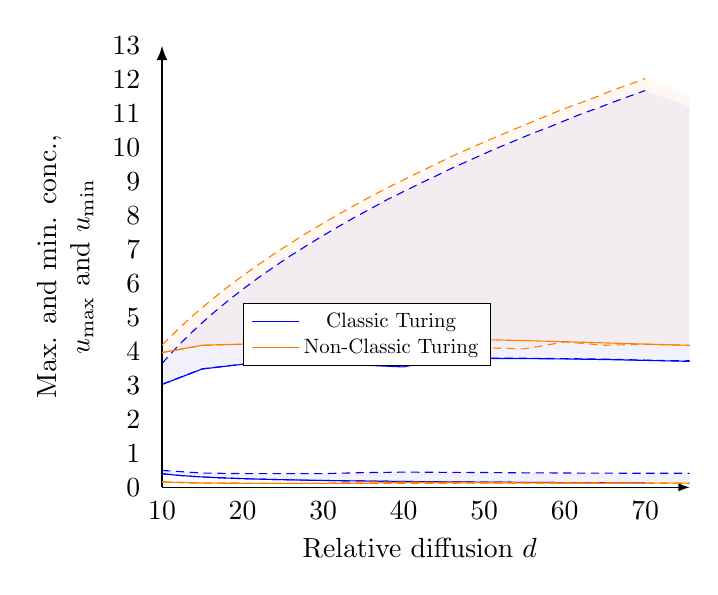
\begin{tikzpicture}
\begin{axis}[
    %hide axis,
    %axis lines* = left,
    %axis lines=left, xtick=\empty, ytick=\empty.
    axis line style={draw=none},
    tick style={draw=none},
    xticklabel style={yshift=-0.1mm},
    xmin = 8.5,
   xmax =75.5,
   ymin = -0.1,
    ymax = 13.1,
    %grid=both,
    %xtick = {1,0.95,...,0.6},
    ytick = {0,1,...,20},    
    %xticklabels = {{zero},$\alpha$,$\varphi$},
   %xlabel style={at={(axis cs:0.61,7)},anchor=east,align=center},
    %ylabel style={at={(axis cs:1.00,35)},anchor=north,rotate=0},
	xlabel = {Relative diffusion $d$},
        ylabel = {Max. and min. conc.,\\ $u_{\max}$ and $u_{\min}$},
        ylabel style = {align=center},
    legend style={at={(axis cs:20,4.5)},anchor=west,cells={align=center},nodes={scale=0.75}},
    %x dir=reverse
    %legend entries = {Decreasing the inactivation rate $k_{-2}$}
]
%-------------------------------------------------------------------------------------------------
% AXES
\draw[->,-latex, thick] (axis cs: 10,0) -- (axis cs: 10,13.0); % y-axis
\draw[->,-latex] (axis cs: 10,0) -- (axis cs: 75.5,0); % x-axis
%-------------------------------------------------------------------------------------------------
%-------------------------------------------------------------------------------------------------
% Classical 
%-------------------------------------------------------------------------------------------------
\addplot[forget plot,densely dashed,color=blue,name path=UpuMaxClassical] coordinates {
		(10.0000	,	3.0340	)
		(15.0000	,	3.4887	)
		(20.0000	,	3.6270	)
		(25.0000	,	3.6538	)
		(30.0000	,	3.6422	)
		(35.0000	,	3.6973	)
		(40.0000	,	3.7671	)
		(45.0000	,	3.7875	)
		(50.0000	,	3.8026	)
		(55.0000	,	3.7999	)
		(60.0000	,	3.7900	)
		(65.0000	,	3.7728	)
		(70.0000	,	3.7468	)
		(75.0000	,	3.7224	)
		(80.0000	,	3.8224	)
		(85.0000	,	3.8307	)
		(90.0000	,	3.8264	)
		(95.0000	,	3.8295	)
		(100.0000	,	3.8623	)
		(105.0000	,	3.8687	)
		(110.0000	,	3.8541	)
		(115.0000	,	3.8648	)
		(120.0000	,	3.8540	)
		(125.0000	,	3.8477	)
		(130.0000	,	3.8396	)
		(135.0000	,	3.8310	)
		(140.0000	,	3.8226	)
		(145.0000	,	3.8679	)
		(150.0000	,	3.8808	)
		(155.0000	,	3.8971	)
		(160.0000	,	3.9024	)
};

\addplot[forget plot,color=blue] coordinates {
		(10.0000	,	3.0280	)
		(15.0000	,	3.4843	)
		(20.0000	,	3.6229	)
		(25.0000	,	3.6510	)
		(30.0000	,	3.6383	)
		(35.0000	,	3.5973	)
		(40.0000	,	3.5449	)
		(45.0000	,	3.7783	)
		(50.0000	,	3.7942	)
		(55.0000	,	3.7913	)
		(60.0000	,	3.7804	)
		(65.0000	,	3.7624	)
		(70.0000	,	3.7378	)
		(75.0000	,	3.7118	)
		(80.0000	,	3.6826	)
		(85.0000	,	3.6535	)
		(90.0000	,	3.6163	)
		(95.0000	,	3.8114	)
		(100.0000	,	3.7967	)
		(105.0000	,	3.7857	)
		(110.0000	,	3.7684	)
		(115.0000	,	3.8476	)
		(120.0000	,	3.8417	)
		(125.0000	,	3.8365	)
		(130.0000	,	3.8295	)
		(135.0000	,	3.8191	)
		(140.0000	,	3.8126	)
		(145.0000	,	3.7996	)
		(150.0000	,	3.7839	)
		(155.0000	,	3.7728	)
		(160.0000	,	3.7590	)
};

\addplot[forget plot,densely dashed,color=blue,name path=DownuMaxClassical] coordinates {
		(10.0000	,	3.6475	)
		(12.0000	,	4.1694	)
		(14.0000	,	4.6316	)
		(16.0000	,	5.0624	)
		(18.0000	,	5.4572	)
		(20.0000	,	5.8282	)
		(22.0000	,	6.1781	)
		(24.0000	,	6.5063	)
		(26.0000	,	6.8264	)
		(28.0000	,	7.1222	)
		(30.0000	,	7.4115	)
		(32.0000	,	7.6902	)
		(34.0000	,	7.9597	)
		(36.0000	,	8.2160	)
		(38.0000	,	8.4758	)
		(40.0000	,	8.7102	)
		(42.0000	,	8.9413	)
		(44.0000	,	9.1679	)
		(46.0000	,	9.3962	)
		(48.0000	,	9.6101	)
		(50.0000	,	9.8220	)
		(52.0000	,	10.0284	)
		(54.0000	,	10.2237	)
		(56.0000	,	10.4223	)
		(58.0000	,	10.6012	)
		(60.0000	,	10.7954	)
		(62.0000	,	10.9888	)
		(64.0000	,	11.1594	)
		(66.0000	,	11.3399	)
		(68.0000	,	11.5134	)
		(70.0000	,	11.6838	)
};
\addplot[blue!50,opacity=0.1,forget plot] fill between[of=UpuMaxClassical and DownuMaxClassical];

\addplot[forget plot,densely dashed,color=blue,name path=UpuMinClassical] coordinates {
		(10.0000	,	0.4980	)
		(15.0000	,	0.4210	)
		(20.0000	,	0.4041	)
		(25.0000	,	0.4020	)
		(30.0000	,	0.4047	)
		(35.0000	,	0.4327	)
		(40.0000	,	0.4479	)
		(45.0000	,	0.4420	)
		(50.0000	,	0.4361	)
		(55.0000	,	0.4275	)
		(60.0000	,	0.4220	)
		(65.0000	,	0.4174	)
		(70.0000	,	0.4145	)
		(75.0000	,	0.4133	)
		(80.0000	,	0.4118	)
		(85.0000	,	0.4115	)
		(90.0000	,	0.4110	)
		(95.0000	,	0.4110	)
		(100.0000	,	0.4122	)
		(105.0000	,	0.4120	)
		(110.0000	,	0.4086	)
		(115.0000	,	0.4098	)
		(120.0000	,	0.4111	)
		(125.0000	,	0.4122	)
		(130.0000	,	0.4134	)
		(135.0000	,	0.4144	)
		(140.0000	,	0.4153	)
		(145.0000	,	0.4081	)
		(150.0000	,	0.4062	)
		(155.0000	,	0.4071	)
		(160.0000	,	0.4063	)
};

\addplot[color=blue] coordinates {
		(10.0000	,	0.4019	)
		(12.0000	,	0.3537	)
		(14.0000	,	0.3195	)
		(16.0000	,	0.2935	)
		(18.0000	,	0.2732	)
		(20.0000	,	0.2563	)
		(22.0000	,	0.2423	)
		(24.0000	,	0.2303	)
		(26.0000	,	0.2200	)
		(28.0000	,	0.2109	)
		(30.0000	,	0.2029	)
		(32.0000	,	0.1956	)
		(34.0000	,	0.1891	)
		(36.0000	,	0.1833	)
		(38.0000	,	0.1779	)
		(40.0000	,	0.1730	)
		(42.0000	,	0.1686	)
		(44.0000	,	0.1644	)
		(46.0000	,	0.1605	)
		(48.0000	,	0.1568	)
		(50.0000	,	0.1535	)
		(52.0000	,	0.1503	)
		(54.0000	,	0.1473	)
		(56.0000	,	0.1445	)
		(58.0000	,	0.1419	)
		(60.0000	,	0.1394	)
		(62.0000	,	0.1370	)
		(64.0000	,	0.1347	)
		(66.0000	,	0.1326	)
		(68.0000	,	0.1305	)
		(70.0000	,	0.1286	)
};

\addplot[forget plot,densely dashed,color=blue,name path=DownuMinClassical] coordinates {
		(10.0000	,	0.4009	)
		(12.0000	,	0.3529	)
		(14.0000	,	0.3190	)
		(16.0000	,	0.2931	)
		(18.0000	,	0.2728	)
		(20.0000	,	0.2560	)
		(22.0000	,	0.2421	)
		(24.0000	,	0.2301	)
		(26.0000	,	0.2198	)
		(28.0000	,	0.2108	)
		(30.0000	,	0.2027	)
		(32.0000	,	0.1955	)
		(34.0000	,	0.1890	)
		(36.0000	,	0.1831	)
		(38.0000	,	0.1778	)
		(40.0000	,	0.1729	)
		(42.0000	,	0.1684	)
		(44.0000	,	0.1642	)
		(46.0000	,	0.1603	)
		(48.0000	,	0.1567	)
		(50.0000	,	0.1533	)
		(52.0000	,	0.1501	)
		(54.0000	,	0.1472	)
		(56.0000	,	0.1444	)
		(58.0000	,	0.1418	)
		(60.0000	,	0.1393	)
		(62.0000	,	0.1369	)
		(64.0000	,	0.1346	)
		(66.0000	,	0.1325	)
		(68.0000	,	0.1305	)
		(70.0000	,	0.1285	)
};
\addplot[blue!50,opacity=0.1,forget plot] fill between[of=UpuMinClassical and DownuMinClassical];

\addlegendentry{Classic Turing}% Add to legend
%-------------------------------------------------------------------------------------------------
% Non-classical
%-------------------------------------------------------------------------------------------------
\addplot[forget plot,densely dashed,color=orange,name path=UpuMaxNonClassical] coordinates {
		(10.0000	,	4.1878	)
		(12.0000	,	4.6571	)
		(14.0000	,	5.0925	)
		(16.0000	,	5.4905	)
		(18.0000	,	5.8700	)
		(20.0000	,	6.2289	)
		(22.0000	,	6.5641	)
		(24.0000	,	6.8880	)
		(26.0000	,	7.1961	)
		(28.0000	,	7.4935	)
		(30.0000	,	7.7764	)
		(32.0000	,	8.0500	)
		(34.0000	,	8.3158	)
		(36.0000	,	8.5724	)
		(38.0000	,	8.8221	)
		(40.0000	,	9.0575	)
		(42.0000	,	9.2867	)
		(44.0000	,	9.5157	)
		(46.0000	,	9.7485	)
		(48.0000	,	9.9577	)
		(50.0000	,	10.1675	)
		(52.0000	,	10.3692	)
		(54.0000	,	10.5683	)
		(56.0000	,	10.7639	)
		(58.0000	,	10.9618	)
		(60.0000	,	11.1531	)
		(62.0000	,	11.3225	)
		(64.0000	,	11.5024	)
		(66.0000	,	11.6954	)
		(68.0000	,	11.8583	)
		(70.0000	,	12.0386	)
};

\addplot[forget plot,color=orange] coordinates {
		(10.0000	,	3.9685	)
		(15.0000	,	4.1835	)
		(20.0000	,	4.2159	)
		(25.0000	,	4.1861	)
		(30.0000	,	4.1289	)
		(35.0000	,	4.0629	)
		(40.0000	,	4.3758	)
		(45.0000	,	4.3700	)
		(50.0000	,	4.3481	)
		(55.0000	,	4.3198	)
		(60.0000	,	4.2874	)
		(65.0000	,	4.2526	)
		(70.0000	,	4.2183	)
		(75.0000	,	4.1845	)
		(80.0000	,	4.1653	)
		(85.0000	,	4.3695	)
		(90.0000	,	4.3482	)
		(95.0000	,	4.3237	)
		(100.0000	,	4.2999	)
		(105.0000	,	4.4090	)
		(110.0000	,	4.2621	)
		(115.0000	,	4.3756	)
		(120.0000	,	4.3681	)
		(125.0000	,	4.3544	)
		(130.0000	,	4.3340	)
		(135.0000	,	4.3179	)
		(140.0000	,	4.3017	)
		(145.0000	,	4.2838	)
		(150.0000	,	4.2741	)
		(155.0000	,	4.2566	)
		(160.0000	,	4.4399	)
};

\addplot[forget plot,densely dashed,color=orange,name path=DownuMaxNonClassical] coordinates {
		(10.0000	,	3.9646	)
		(15.0000	,	4.1802	)
		(20.0000	,	4.2116	)
		(25.0000	,	4.1832	)
		(30.0000	,	4.1223	)
		(35.0000	,	4.0588	)
		(40.0000	,	3.9997	)
		(45.0000	,	3.9520	)
		(50.0000	,	4.1073	)
		(55.0000	,	4.0750	)
		(60.0000	,	4.2822	)
		(65.0000	,	4.1838	)
		(70.0000	,	4.2132	)
		(75.0000	,	4.1785	)
		(80.0000	,	4.1480	)
		(85.0000	,	4.1249	)
		(90.0000	,	4.0982	)
		(95.0000	,	4.0698	)
		(100.0000	,	4.0525	)
		(105.0000	,	4.2704	)
		(110.0000	,	4.1215	)
		(115.0000	,	4.2239	)
		(120.0000	,	4.2109	)
		(125.0000	,	4.0682	)
		(130.0000	,	4.1868	)
		(135.0000	,	4.2322	)
		(140.0000	,	4.2931	)
		(145.0000	,	4.2769	)
		(150.0000	,	4.1496	)
		(155.0000	,	4.1892	)
		(160.0000	,	4.2343	)
};
\addplot[orange!50,opacity=0.1,forget plot] fill between[of=UpuMaxNonClassical and DownuMaxNonClassical];

\addplot[forget plot,densely dashed,color=orange,name path=UpuMinNonClassical] coordinates {
		(10.0000	,	0.1584	)
		(15.0000	,	0.1260	)
		(20.0000	,	0.1183	)
		(25.0000	,	0.1165	)
		(30.0000	,	0.1168	)
		(35.0000	,	0.1615	)
		(40.0000	,	0.1510	)
		(45.0000	,	0.1461	)
		(50.0000	,	0.1393	)
		(55.0000	,	0.1335	)
		(60.0000	,	0.1297	)
		(65.0000	,	0.1274	)
		(70.0000	,	0.1250	)
		(75.0000	,	0.1230	)
		(80.0000	,	0.1217	)
		(85.0000	,	0.1207	)
		(90.0000	,	0.1229	)
		(95.0000	,	0.1245	)
		(100.0000	,	0.1232	)
		(105.0000	,	0.1222	)
		(110.0000	,	0.1213	)
		(115.0000	,	0.1204	)
		(120.0000	,	0.1196	)
		(125.0000	,	0.1190	)
		(130.0000	,	0.1187	)
		(135.0000	,	0.1189	)
		(140.0000	,	0.1182	)
		(145.0000	,	0.1178	)
		(150.0000	,	0.1194	)
		(155.0000	,	0.1254	)
		(160.0000	,	0.1245	)
};

\addplot[color=orange] coordinates {
		(10.0000	,	0.1579	)
		(15.0000	,	0.1258	)
		(20.0000	,	0.1181	)
		(25.0000	,	0.1164	)
		(30.0000	,	0.1166	)
		(35.0000	,	0.1174	)
		(40.0000	,	0.1483	)
		(45.0000	,	0.1423	)
		(50.0000	,	0.1364	)
		(55.0000	,	0.1320	)
		(60.0000	,	0.1283	)
		(65.0000	,	0.1257	)
		(70.0000	,	0.1239	)
		(75.0000	,	0.1224	)
		(80.0000	,	0.1209	)
		(85.0000	,	0.1179	)
		(90.0000	,	0.1177	)
		(95.0000	,	0.1177	)
		(100.0000	,	0.1177	)
		(105.0000	,	0.1212	)
		(110.0000	,	0.1180	)
		(115.0000	,	0.1192	)
		(120.0000	,	0.1191	)
		(125.0000	,	0.1185	)
		(130.0000	,	0.1182	)
		(135.0000	,	0.1180	)
		(140.0000	,	0.1177	)
		(145.0000	,	0.1175	)
		(150.0000	,	0.1174	)
		(155.0000	,	0.1174	)
		(160.0000	,	0.1181	)
};

\addplot[forget plot,densely dashed,color=orange,name path=DownuMinNonClassical] coordinates {
		(10.0000	,	0.1572	)
		(15.0000	,	0.1257	)
		(20.0000	,	0.1180	)
		(25.0000	,	0.1164	)
		(30.0000	,	0.1166	)
		(35.0000	,	0.1174	)
		(40.0000	,	0.1185	)
		(45.0000	,	0.1195	)
		(50.0000	,	0.1271	)
		(55.0000	,	0.1256	)
		(60.0000	,	0.1273	)
		(65.0000	,	0.1199	)
		(70.0000	,	0.1210	)
		(75.0000	,	0.1185	)
		(80.0000	,	0.1179	)
		(85.0000	,	0.1176	)
		(90.0000	,	0.1175	)
		(95.0000	,	0.1176	)
		(100.0000	,	0.1176	)
		(105.0000	,	0.1177	)
		(110.0000	,	0.1178	)
		(115.0000	,	0.1180	)
		(120.0000	,	0.1182	)
		(125.0000	,	0.1183	)
		(130.0000	,	0.1177	)
		(135.0000	,	0.1175	)
		(140.0000	,	0.1174	)
		(145.0000	,	0.1172	)
		(150.0000	,	0.1172	)
		(155.0000	,	0.1171	)
		(160.0000	,	0.1170	)
};
\addplot[orange!50,opacity=0.1,forget plot] fill between[of=UpuMinNonClassical and DownuMinNonClassical];

\addlegendentry{Non-Classic Turing}% Add to legend
\end{axis}

\end{tikzpicture}



\end{document}
